\documentclass{article} % For LaTeX2e
\usepackage{graphicx}
\usepackage{final_project,times}
%\documentstyle[nips12submit_09,times,art10]{article} % For LaTeX 2.09
\usepackage{csvsimple}


\begin{filecontents*}{grade.csv}
name,givenname,matriculation,gender,grade
Maier,Hans,12345,m,1.0
Huber,Anna,23456,f,2.3
Weisbaeck,Werner,34567,m,5.0
\end{filecontents*}
\begin{filecontents*}{114.csv}
a,b,c,d,e
"MURKOWSKI (R-AK)",0.497598664894792,0.273265644364143,0.855263157894737,0.0427631578947368
"COCHRAN (R-MS)",0.419582376565703,0.239057683547413,0.855263157894737,0.00986842105263158
"CAPITO (R-WV)",0.419130425638844,0.247081733551818,0.868421052631579,0.00657894736842105
"ALEXANDER (R-TN)",0.41438661703442,0.220710476818469,0.835526315789474,0.0328947368421053
"AYOTTE (R-NH)",0.40000077106231,0.246194491337452,0.878289473684211,0.00328947368421053
"MCCAIN (R-AZ)",0.397691117971077,0.216653114623947,0.842105263157895,0.0296052631578947
"CORKER (R-TN)",0.394670224734382,0.204932618186271,0.822368421052632,0.0361842105263158
"GRAHAM (R-SC)",0.379954663910313,0.158065667276924,0.641447368421053,0.286184210526316
"HATCH (R-UT)",0.376092397149784,0.210037860216363,0.845394736842105,0.00986842105263158
"ROUNDS (R-SD)",0.37176078200335,0.213203161101553,0.851973684210526,0.00657894736842105
"KIRK (R-IL)",0.368321820672167,0.185841750906516,0.809210526315789,0.0625
"JOHNSON (R-WI)",0.360464638064774,0.207682754121955,0.851973684210526,0.00657894736842105
"PORTMAN (R-OH)",0.358130096569216,0.204173829508763,0.851973684210526,0.0164473684210526
"FLAKE (R-AZ)",0.358087792663536,0.18047081738718,0.802631578947368,0.0361842105263158
"GARDNER (R-CO)",0.330339183259192,0.175729543832057,0.822368421052632,0.0197368421052632
"THUNE (R-SD)",0.32948322650275,0.182887932883591,0.835526315789474,0.00986842105263158
"COLLINS (R-ME)",0.327897733790534,0.191294202337041,0.848684210526316,0
"BURR (R-NC)",0.316590283173148,0.173451832999668,0.825657894736842,0.00657894736842105
"CORNYN (R-TX)",0.310158896567386,0.172759128460187,0.828947368421053,0.00328947368421053
"TILLIS (R-NC)",0.310015063025369,0.174909834599211,0.828947368421053,0
"HOEVEN (R-ND)",0.305440608516977,0.169189939903801,0.828947368421053,0.00657894736842105
"COATS (R-IN)",0.303485065174123,0.158111699467533,0.802631578947368,0.0131578947368421
"HELLER (R-NV)",0.292931348727467,0.149129205715818,0.802631578947368,0.0296052631578947
"ENZI (R-WY)",0.289137349124391,0.141262479972827,0.789473684210526,0.0427631578947368
"ROBERTS (R-KS)",0.284198527457331,0.150017805165135,0.805921052631579,0.00986842105263158
"WICKER (R-MS)",0.279000974925311,0.145719881106983,0.802631578947368,0.0131578947368421
"ISAKSON (R-GA)",0.277565695070196,0.149565416360703,0.8125,0.00657894736842105
"ERNST (R-IA)",0.261037314512154,0.143316411211595,0.809210526315789,0
"FISCHER (R-NE)",0.258076734124903,0.139420406279785,0.799342105263158,0
"SCOTT (R-SC)",0.256729338862997,0.12788932626296,0.776315789473684,0.0197368421052632
"MCCONNELL (R-KY)",0.254988341847377,0.136531982806693,0.792763157894737,0
"CASSIDY (R-LA)",0.253761595296395,0.129648651173199,0.789473684210526,0.0164473684210526
"BARASSO (R-WY)",0.25068871541465,0.137167897255826,0.805921052631579,0
"BLUNT (R-MO)",0.246217417608855,0.115233996565166,0.746710526315789,0.0427631578947368
"TOOMEY (R-PA)",0.238746001991062,0.108294999623425,0.736842105263158,0.0592105263157895
"MORAN (R-KS)",0.238689724062656,0.111318720286692,0.75,0.0427631578947368
"SULLIVAN (R-AK)",0.231272297569466,0.113267286773937,0.773026315789474,0.0263157894736842
"PERDUE (R-GA)",0.229140912783247,0.119891955679491,0.773026315789474,0
"DAINES (R-MT)",0.222145612643784,0.118899809836637,0.789473684210526,0
"GRASSLEY (R-IA)",0.221257362207501,0.119982744566244,0.796052631578947,0
"BOOZMAN (R-AR)",0.215410894795523,0.109303371250294,0.773026315789474,0.00986842105263158
"INHOFE (R-OK)",0.211186302549713,0.106733482055432,0.769736842105263,0.00986842105263158
"LANKFORD (R-OK)",0.203616995455809,0.105762834582707,0.766447368421053,0
"COTTON (R-AR)",0.174392614905796,0.084845931359294,0.733552631578947,0.00986842105263158
"RISCH (R-ID)",0.17371081113549,0.0854969721552683,0.736842105263158,0.00657894736842105
"SASSE (R-NE)",0.16352622486792,0.079793629106398,0.726973684210526,0.00657894736842105
"CRAPO (R-ID)",0.157660465164756,0.0737465021611789,0.723684210526316,0.0230263157894737
"SESSIONS (R-AL)",0.153693450380507,0.0733305609516371,0.723684210526316,0.0131578947368421
"VITTER (R-LA)",0.142889367537259,0.0557764369500126,0.625,0.171052631578947
"SHELBY (R-AL)",0.133824045732276,0.06166173146231,0.697368421052632,0.0197368421052632
"LEE (R-UT)",0.13108742096644,0.055046727784959,0.651315789473684,0.0657894736842105
"PAUL (R-KY)",0.113233692637549,0.0474315169055174,0.648026315789474,0.0625
"RUBIO (R-FL)",0.10486230534523,0.0381832705258285,0.476973684210526,0.351973684210526
"CRUZ (R-TX)",0.0978418179736759,0.0357198518208409,0.526315789473684,0.246710526315789
"MANCHIN (D-WV)",0.0799038003906862,0.0372870691721282,0.694078947368421,0.0164473684210526
"HEITKAMP (D-ND)",0.0617163992312076,0.0305416881726838,0.694078947368421,0
"SANDERS (I-VT)",0.051795954021323,0.0217529651493747,0.421052631578947,0.0427631578947368
"MCCASKILL (D-MO)",0.0426841141191478,0.0188628005108972,0.625,0.0296052631578947
"MARKEY (D-MA)",0.0396078761329401,0.0171037960467209,0.4375,0.0263157894736842
"DONNELLY (D-IN)",0.0336043523953942,0.0157539006121219,0.657894736842105,0.00986842105263158
"BROWN (D-OH)",0.0295905735659886,0.0129296760844992,0.453947368421053,0.0197368421052632
"FRANKEN (D-MN)",0.0286842918593299,0.0124929882170023,0.467105263157895,0.0230263157894737
"WARREN (D-MA)",0.0278689427137122,0.0129460215160472,0.444078947368421,0
"BOOKER (D-NJ)",0.0267751889254905,0.0120087243840037,0.457236842105263,0.00986842105263158
"MERKLEY (D-OR)",0.026564447937852,0.0118973897389871,0.447368421052632,0.00986842105263158
"MENENDEZ (D-NJ)",0.0264528091363982,0.011603670788684,0.470394736842105,0.0197368421052632
"COONS (D-DE)",0.025369712363465,0.0107771600715256,0.503289473684211,0.0394736842105263
"GILLIBRAND (D-NY)",0.0243855023134967,0.0111638314495326,0.457236842105263,0.00328947368421053
"LEAHY (D-VT)",0.0226584106941522,0.010174584385679,0.470394736842105,0.00986842105263158
"UDALL (D-NM)",0.0190988945883588,0.00856252504919017,0.476973684210526,0.00986842105263158
"BALDWIN (D-WI)",0.0189638068160024,0.00881930189013577,0.470394736842105,0
"SCHUMER (D-NY)",0.016930402070906,0.0076654489146292,0.480263157894737,0.00657894736842105
"BLUMENTHAL (D-CT)",0.0169280288026104,0.00778100663882319,0.496710526315789,0.00328947368421053
"HIRONO (D-HI)",0.0156321753561577,0.00715486499081908,0.480263157894737,0.00328947368421053
"DURBIN (D-IL)",0.0151563596368044,0.00689635671659457,0.493421052631579,0.00657894736842105
"BOXER (D-CA)",0.0150389151151139,0.00579943242914295,0.440789473684211,0.105263157894737
"REED (D-RI)",0.0144628601230646,0.00669705937629966,0.473684210526316,0
"SCHATZ (D-HI)",0.0143497628981308,0.00645584192720127,0.496710526315789,0.00986842105263158
"CARDIN (D-MD)",0.0142484933725278,0.00664135397443045,0.486842105263158,0
"PETERS (D-MI)",0.01328432903134,0.00592056175103579,0.503289473684211,0.0131578947368421
"WYDEN (D-OR)",0.0125173364696578,0.00564684623528758,0.486842105263158,0.00657894736842105
"MURPHY (D-CT)",0.0112985496275971,0.00508662817486303,0.486842105263158,0.00657894736842105
"HEINRICH (D-NM)",0.0110404234286951,0.00500382969674257,0.5,0.00657894736842105
"MURRAY (D-WA)",0.0106841610767782,0.00476998325712272,0.532894736842105,0.0164473684210526
"WARNER (D-VA)",0.00732211717008343,0.00311443603253109,0.569078947368421,0.0328947368421053
"STABENOW (D-MI)",0.00729164941348994,0.00324108704723413,0.509868421052632,0.0131578947368421
"NELSON (D-FL)",0.00567368965979241,0.00224540038886134,0.490131578947368,0.0756578947368421
"SHAHEEN (D-NH)",0.00474610501754609,0.00217031622443339,0.539473684210526,0.00657894736842105
"WHITEHOUSE (D-RI)",0.00447920499053952,0.00206915935024362,0.503289473684211,0
"KLOBUCHAR (D-MN)",0.00418618125066623,0.00190168422935224,0.536184210526316,0.00657894736842105
"KAINE (D-VA)",0.0039767684677456,0.00182905465128967,0.572368421052632,0.00328947368421053
"KING (I-ME)",0.00388831053850942,0.0016532480441568,0.552631578947368,0.0328947368421053
"FEINSTEIN (D-CA)",0.00326170653063853,0.00138959685038929,0.5625,0.0328947368421053
"CANTWELL (D-WA)",0.00286004788780935,0.00134154704819968,0.532894736842105,0
"MIKULSKI (D-MD)",0.00284014613985294,0.00115937695363105,0.480263157894737,0.0493421052631579
"TESTER (D-MT)",0.00277193568051751,0.00126846825215361,0.559210526315789,0.00328947368421053
"REID (D-NV)",0.00271896548384673,0.000980928857989217,0.414473684210526,0.184210526315789
"CARPER (D-DE)",0.00244761324753105,0.00108040848345837,0.555921052631579,0.0131578947368421
"BENNET (D-CO)",0.00238434892855792,0.00113176053794164,0.592105263157895,0
"CASEY (D-PA)",0.00220779788075772,0.00101113528961795,0.536184210526316,0.00328947368421053

\end{filecontents*}

\title{Analyzing Senator Community Structure from 2012-2015 Roll Call Data}


\author{
Weiwei Li$^1$, Zhengling Qi$^1$, Yuzhou Sun$^2$, Wenting Hu$^2$\\
%\thanks{ Use footnote for providing further information
%about author (webpage, alternative address)} \\
$^1$Department of Statistics and Operations Research, the University of North Carolina, Chapel Hill, NC 27708\\ 
$^2$Departments of Electrical and Computer Engineering, Duke University, Durham, NC 27708\\
%\texttt{weiweili@live.unc.edu)}\\\texttt{zq15@duke.edu}\\\texttt{yuzhou.sun@duke.edu}\\\texttt{wenting.hu@duke.edu}\\
}

\newcommand{\fix}{\marginpar{FIX}}
\newcommand{\new}{\marginpar{NEW}}

\nipsfinalcopy

\begin{document}


\maketitle

\begin{abstract}
 In this project, we analyzed the 111th-114th roll calls in the US Senate (2012-2015), by applying unsupervised learning methods to assess the association between pairs of senators based on the votes they cast. For pairs, we used similarity-based methods, including hierarchical clustering and multidimensional scaling. We also applied information entropy to find the most influential senators during these periods. By doing so, we observed the gap between Democratic Party and Republican Party increases with time. The senators? goal and behavior is more and more consistent to their representative party.
\end{abstract}

\section{Introduction}
Roll call data is popular in politics that is well - amenable to detect community structure among senators by data mining techniques. In our research, we downloaded roll call voting results from voteview.com, which is supported by researchers from Berkeley, Princeton and San Diego. For each roll call, the txt file provides a list of votes cast by each of the senators. For each of those, the vote of every senator is recorded in three ways: 'Yea', 'Nay' and 'Not Voting'.

Throughout our project, we are particularly interested in digging out time-varying community structures (aside from the obvious segmentation via Democracy party and Republican Party) behind senators from 2012-2015, which can better describe the voting behaviors of senators.

Basically, we use Rajski's distance[1] to evaluate pairs of senator's distance which enjoys the universal metric property. Based on the distance matrix, we first make use of hierarchical clustering without using prior knowledge including party information. In addition, multi-dimensional scaling was conducted to visualize all the senators in Euclidean space, which helps us to further understand the gap between senators. After analyzing the overall relationship between senators, we focus on senators individual influence on voting results by three criterions such as agreement ratio and information share rate.

Rajski's distance is widely used in information science, particular for categorical data since entropy estimation for continuous variable is hard to approximation. Rajski's distance enjoys universal metric property, which means that when two points are closed in other non-trivial metric distance, they will be also close under Rajski's distance.
Multidimensional scaling is a technique of visualizing the level of similarity of objects with high dimensional features. It refers to a set of related coordination techniques used in information science by using distance matrix. In our project, we apply metric measure to multidimensional scaling instead of non-metric measure.

In Section 2 we define Rajski's distance and its property. In section3, we perform hierarchical clustering and 2-D multidimensional scaling to detect hidden community structure behind senators. Influential analysis is used to quantify senators' individual impact on issues in Section 4.

\section{Rajski's Distance}
\subsection{Definition of Rajski's Distance}
Since voting result for every senator is a binary vector, we use the information-theoretic Rajski's distance to measure all pairs of senators. It is a metricized version of mutual information which obeys the triangle inequality and other requirement for a metric. Obviously, the larger the Rajski's distance, the more separate the two senators. The Rajski's distance is defined as:
$$d(X,Y)=1-\frac{I(X;Y)}{H{X,Y}}$$
where $H(X,Y)$ is the joint entropy of two random variable X and Y. \\
The mutual information and joint entropy are define as:
$$I(X;Y)=\sum_{y\in Y}\sum_{x\in X}p(x,y)\log\frac{p(x,y)}{p(x)p(y)}$$
$$H(X;Y)=-\sum_{x}\sum_{y}P(x,y)\log_2P(x,y)$$
The assumption behind Rajski's distance is that each senator is regarded as random variable. Besides, by using mutual and joint entropy, independent assumption is made on each issue vote by senators. This strong assumption may be replaced by weakly dependency in future work.
\subsection{Displaying Dissimilarity Matrices}
Rajski's distance as plain numbers provides little insight. However, we can provide the distances between all pairs of senators in the form of a graphical matrix. The symmetric dissimilarity matrix graphically illustrates the information-theoretic Rajski's distance between all pairs of senators, based on their votes. If two senators voted similarly, the square at the intersection of their names is dark. 
\begin{figure}[h]
\begin{center}
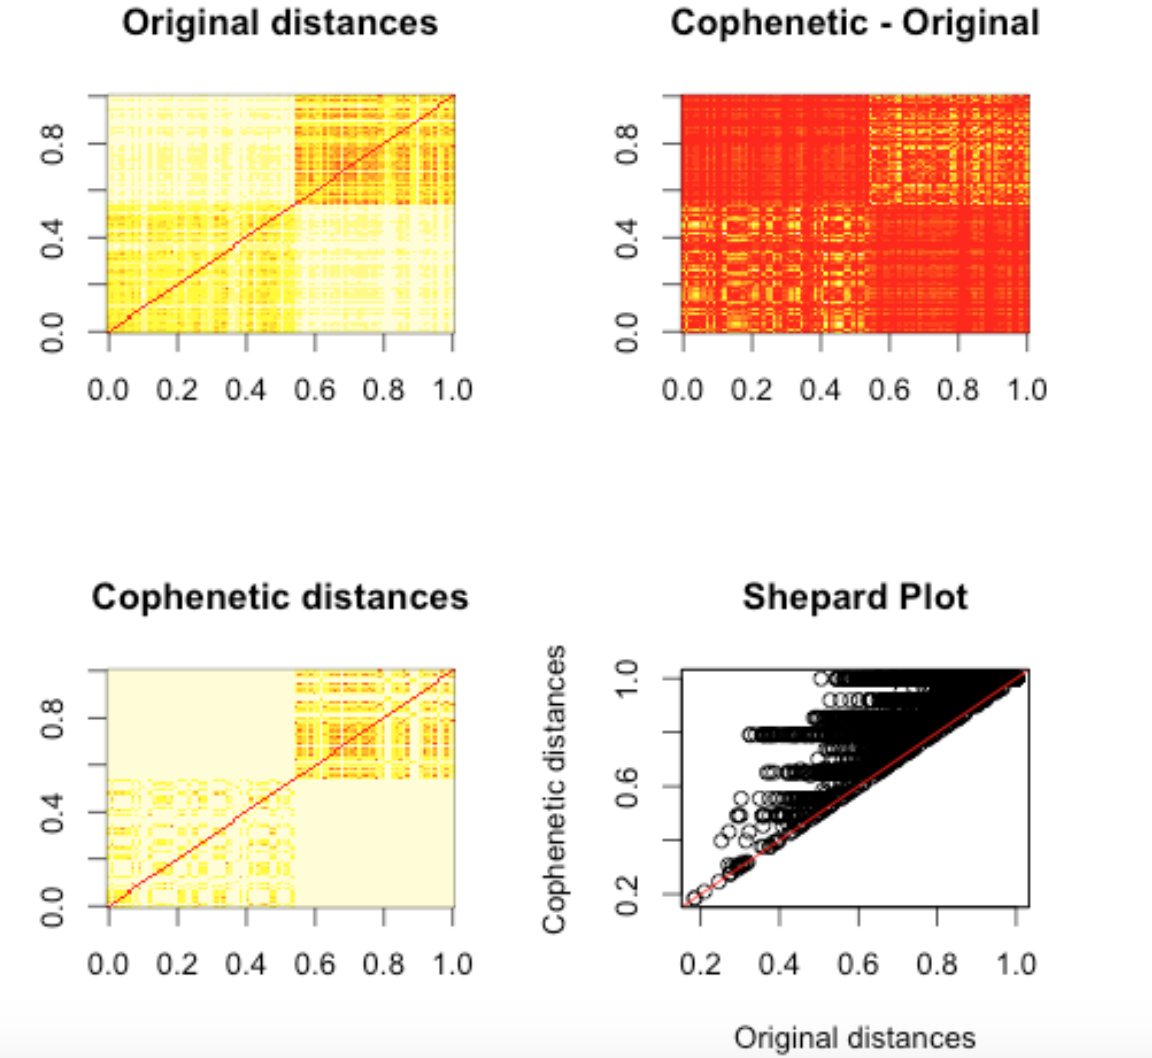
\includegraphics[width=0.5\textwidth]{fig1}
%\fbox{\rule[-.5cm]{0cm}{4cm} \rule[-.5cm]{4cm}{0cm}}
\end{center}
\caption{Dissimilarity Matrices for 111th-114th Senators}
\end{figure}
As we can see from the graph, two large clusters can be identified visually from this graph, and one group of moderate senators in each party. The major clusters correspond to the political parties even if the party information was not used in the computation of distance.
\section{Clustering Analysis}
\subsection{Hierarchical Clustering}
In the hierarchical agglomerative clustering[2] of senators based on their pair-wise Rajski's distance, we can identify the two major clusters: the Republican(green) and the Democratic(red), senators with no party affiliations are marked as blue. An interesting fact is, independent senators seem to have the same preference with Democracy side.

From Figure 2, we observed that as time goes from 2012-2015, the boundary between two parties becomes more and more clear. For example, during 2012-2014, we can still find some senators votes opposite to their belong parties, like Mark Kirk from Illinois in 2012.\\
\begin{figure}[h]
\begin{center}
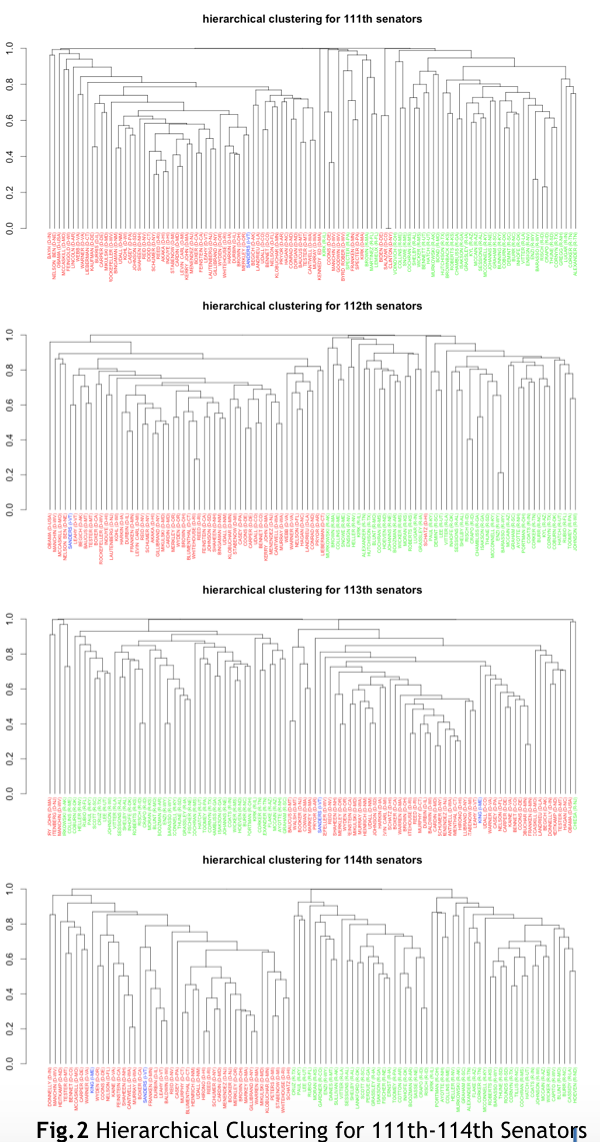
\includegraphics[width=0.5\textwidth]{fig2}
%\fbox{\rule[-.5cm]{0cm}{4cm} \rule[-.5cm]{4cm}{0cm}}
\end{center}
\caption{Hierarchical Clustering for 111th-114th Senators}
\end{figure}
\subsection{Multi-Dimensional Scaling[3]}
To distinguish similarity, which is in our case quantified information-theoretically with a probabilistic model, from distance that is defined geometrically. 

If each senator is denoted with a point in some k-dimensional space, we can try to place these points so that the Euclidean distances between the points would match the distances as specified by the dissimilarity matrix. By using 2-D multi-dimensional scaling, we could visualize the senators in 2-D coordinate(Figure 3).

The senators whose votes were similar, also appear close in the resulting diagrams. From 111th to 114th 2-D multi-dimensional scaling, we again validate our conjecture that the gap between two parties is constantly becoming larger.
\begin{figure}[h]
\begin{center}
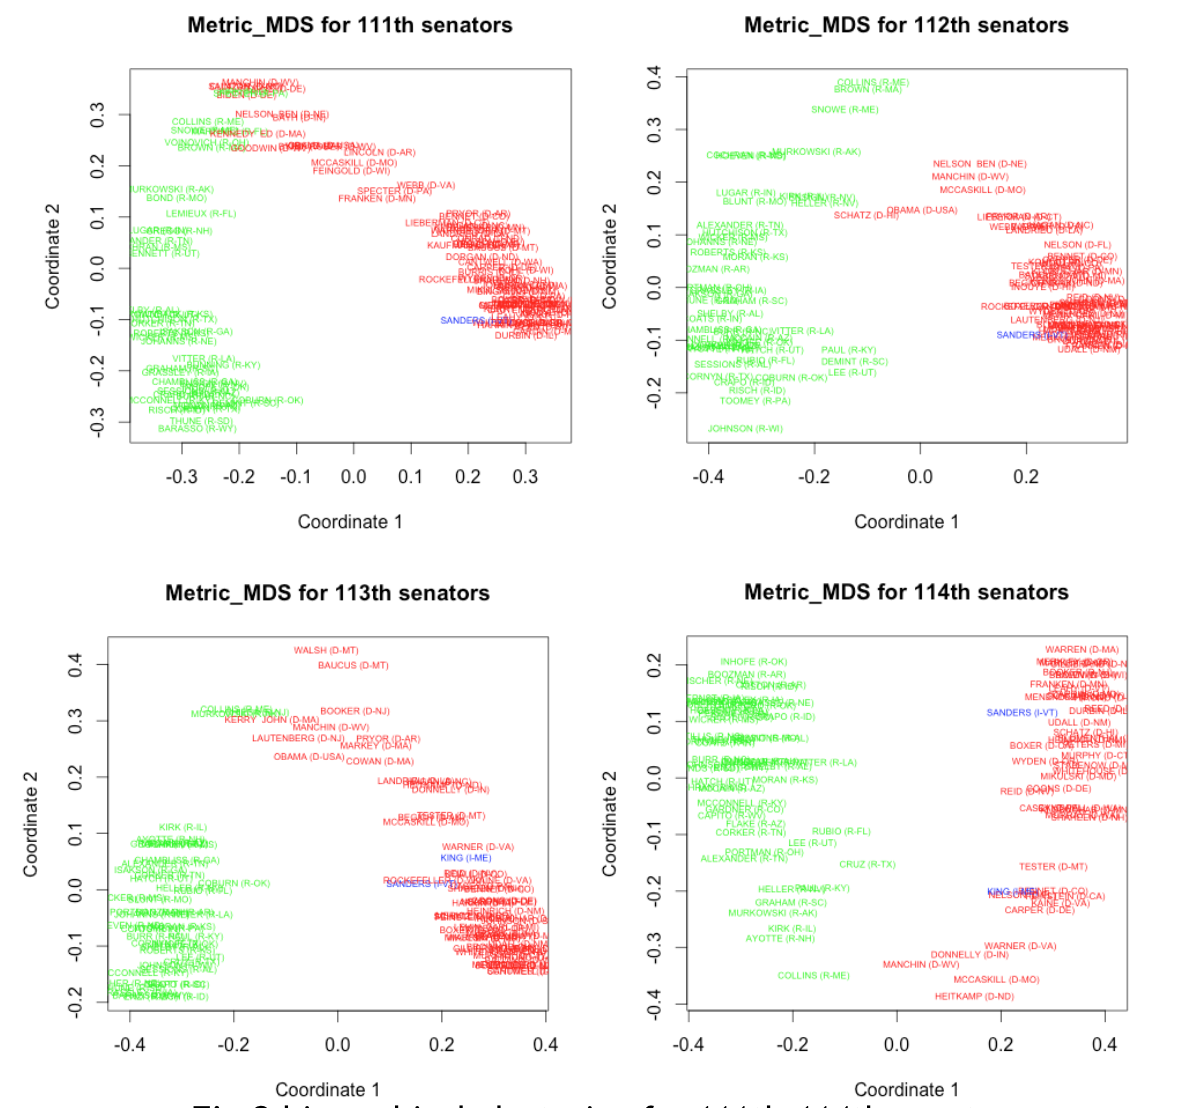
\includegraphics[width=0.5\textwidth]{fig3}
%\fbox{\rule[-.5cm]{0cm}{4cm} \rule[-.5cm]{4cm}{0cm}}
\end{center}
\caption{Multi-Dimensional Scaling for 111th-114th Senators}
\end{figure}
\section{Influential Analysis}
\subsection{Individual Senator Influence Analysis
}
We may define influence as the similarity between a vote cast and the outcome. We can interpret the process of voting under the framework of information theory[1]. Each senator can be considered as an information source, while the outcome of the vote is the destination. Therefore, mutual information can be interpreted as a measure of how influential is a senator with respect to the outcome of the vote.
\begin{center}Table 1: Top 5 Most Influential Senators
\end{center}
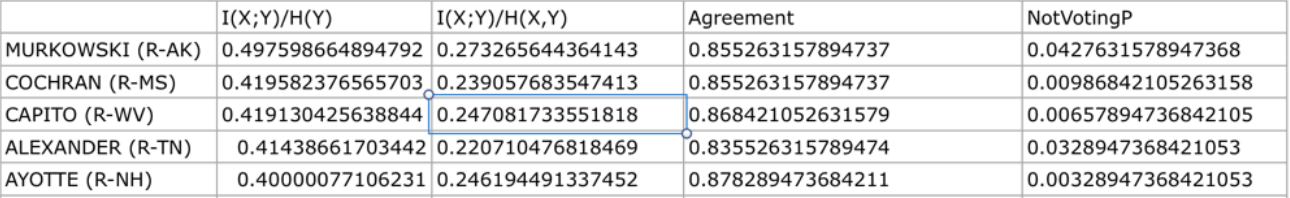
\includegraphics[width=1\textwidth]{table1}

In order to find the influential senators, we use three criterion to evaluate their voting impact. The first one is the percentage of outcome entropy eliminated by the senator's vote, the second one is the percentage of mutual information between outcome and vote eliminated by senator's vote and the last one is the percentage of issues when the vote and the outcome matched. 

Interestingly, from above table, top 5 most influential senators are all from Republican Party. Overall, aggressive assertion could be made that republican senators are more influential than democratic senators. However this criterion should be further investigated based on such as graphical model.

\section{Conclusion}
Roll call data represents senators' political ideologies, which can be used to detect senators' community structure. Therefore, we have investigated the 111th-114th Senate from both a global perspective viewing pairs of senators and viewing voting a local pair-wise perspective within the Senate. That senators from the same party tend to vote similarly and the senators from Republican Party are more influential. In the meantime, we observe a time-varying community structure during the 2012-2015. Basically, the gap between two main parties are becoming larger and larger both from hierarchical clustering and 2-D multidimensional scaling. We found that data analysis methods developed for natural and social sciences were useful also in political science.\\
Our future work could combine voting results and bill questions via topic modeling methods, which could further detect the voting behavior or ideology behind senators.



\subsubsection*{Acknowledgments}

We would like to thank our supervisor, Prof. Sayan Mukherjee, Duke University, for support and tutoring us to work on analyzing senators' roll call data. We also thank the the Voteview Website (http://voteview.com/) providing the data.
\subsubsection*{References}

\small{
[1] A. Jakulin, W. Buntine, T. M. La Pira and H. Brasher {\it
Analyzing the U.S. Senate in 2003: Similarities, Clusters, and Blocs
Political Analysis} 2009 17 (3): 291-310.  

[2] L. Kaufman and P. J. Rousseeuw. {\it Finding Groups in Data: An Introduction to Cluster Analysis}. Wiley, New York, 1990.

[3] J. de Leeuw. {\it Applications of convex analysis to multidimensional scaling}. In J. R. Barra, F. Brodeau, G. Romier, and B. van Cutsem, editors, Recent developments in statistics, pages 133-145, Amsterdam, The Netherlands, 1977. North Holland Publishing Company.

\subsubsection*{Appendix}

    \begin{tabular}{l|c}%
    \bfseries Person & \bfseries Matr.~No.% specify table head
    \csvreader[head to column names]{grade.csv}{}% use head of csv as column names
    {\\\hline\givenname\ \name & \matriculation}% specify your coloumns here
    \end{tabular}
    \\
    114th influential senators.csv\\
    \begin{tabular}{l|cccc}%
    \bfseries Senetor & \bfseries I(X;Y)/H(Y) & \bfseries I(X;Y)/H(X,Y)  & \bfseries Agreement & \bfseries NotVotingP% specify table head
      \csvreader[head to column names]{114.csv}{}% use head of csv as column names
   % specify your coloumns here
    {\\\hline\a & \b & \c & \d & \e}
    \end{tabular}
   % "","I(X;Y)/H(Y)","I(X;Y)/H(X,Y)","Agreement","NotVotingP"
%"MURKOWSKI (R-AK)"
\end{document}
